\documentclass[main.tex]{subfiles}
\begin{document}

\href{https://www2.seas.gwu.edu/~simhaweb/quantum/modules/module1/module1.html}{Module 1}

\begin{enumerate}

\item[] \textbf{In-Class Exercise 1:} \textbf{Q.} What is the shape of the histogram? \textbf{A.} It should be a Gaussian on the $Z$ axis. \textbf{Q} Draw out a potential histogram by completing the histogram above. \textbf{A.} Figure \ref{fig:e01Gaussian}. \textbf{Q.} What would we expect to see with thinner and thinner bands (many of them), and lots of pellets? \textbf{A.} A continuous distribution. \textbf{Q.} If we replaced horizontal bands with vertical bands near the x-axis to get an x-histogram, what would it look like? \textbf{A.} It would also be Gaussian.

\begin{figure}
  \centering
  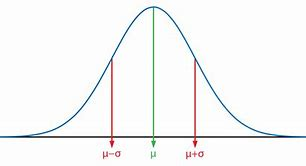
\includegraphics[width=3in]{modules/figs/m01/e01gaussian.jpeg}
  \caption{Gaussian distribution}
  \label{fig:e01Gaussian}
\end{figure}

\item[] \textbf{In-Class Exercise 2:} \textbf{Q.} How would your responses change if we placed a hole-in-a-wall between the gun and the screen? \textbf{A.} A more concentrated distribution.

\item[] \textbf{In-Class Exercise 3:} \textbf{Q.} Now consider moving the pellet gun further back so that the spread of trajectories is wide enough to encompass both holes shown here: What would the x and y histograms look like? And how would those change if we changed holes to slits?

\begin{figure}
  \centering
  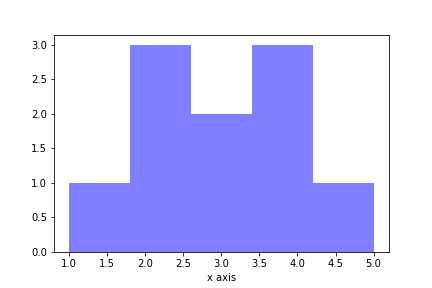
\includegraphics[width=3in]{modules/figs/m01/e03xaxis.png}
  \caption{Two hole X axis Histogram}
  \label{fig:e03xaxis}
\end{figure}

\begin{figure}
  \centering
  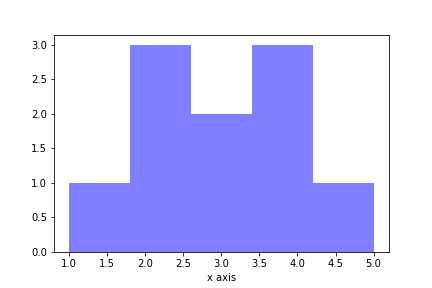
\includegraphics[width=3in]{modules/figs/m01/e03xaxis.png}
  \caption{Two hole Y axis Histogram}
  \label{fig:e03yaxis}
\end{figure}

\item[] \textbf{In-Class Exercise 4:}

    \begin{enumerate}
        \item[1.] What is the source of randomness in each case?
        \item[2.] For the coin-flip, could one in principle, knowing the launch velocity of the coin (and other variables) predict the outcome? What variables would be needed? Could a mechanical contraption be designed to flip a coin predictably?
        \item[3.] Does this predictability extend to the card example?
        \item[4.] What is an example of a physical measurement that is likely to have random errors, and for which an average over several measurements is needed?
    \end{enumerate}

\item[] \textbf{In-Class Exercise 5:} How would you describe the motion of the bar magnet? What is the net force experienced by the center of the bar magnet?

\item[] \textbf{In-Class Exercise 6:} Now how would you describe the motion of the bar magnet? What is the net force experienced by the center of the bar magnet, and why?

\item[] \textbf{In-Class Exercise 7:} What does one expect for the z-histogram (vertical), and why? That is, what is the histogram going to look like if we count the "hits" in each little blue box? If one knows the landing spot for a particular bar magnet, how could one compute the vertical force experienced by the magnet?

\item[] \textbf{In-Class Exercise 8:} What other questions might one ask? What are you curious to know about this type of experiment?

\item[] \textbf{In-Class Exercise 9:} Sketch, with modest neatness, the Type-1 and Type-2 diagrams for a two-stage SG experiment when the orientation of the second apparatus is

    \begin{enumerate}
        \item[1.] $\theta=0$
        \item[2.] $\theta=\pi$
        \item[3.] $\theta=\frac{\pi}{2}$
        \item[4.] $\theta=\frac{\pi}{4}$
    \end{enumerate}

\item[] \textbf{In-Class Exercise 10:} 10: Sketch Type-1 and Type-2 diagrams for a three-stage SG experiment where:

    \begin{enumerate}
        \item[1.] The + output of the first stage is fed into the second.
        \item[2.] The + output of the second stage is fed into a third apparatus.
        \item[3.] The orientations of the three stages are: $\theta_{1}=0$, $\theta_{2}=\frac{\pi}{2}$, $\theta_{3}=0$.
    \end{enumerate}

\item[] \textbf{In-Class Exercise 11:} How does one test that the splitting between two streams is random? Is it enough to merely establish that 50\% exit through the + stream?

\item[] \textbf{In-Class Exercise 12:} Explore the above notion of independence. Why does it matter?

\item[] \textbf{In-Class Exercise 13:} What is a reasonable guess for the probabilities at two rightmost outputs? Start by asking: what is the probability that an atom arrives at the output of the merge apparatus? Then, further, what is the probability of such an atom to appear at the + output of the third stage? What is, therefore, the overall probability that an atom entering the first appears at the + of the third?
[Answer provided in class]

\item[] \textbf{In-Class Exercise 14:} To clarify the orientation of the second SG apparatus, draw the Type-1 diagram for the above case.

\item[] \textbf{In-Class Exercise 15:} What are your own additional questions?

\item[] \textbf{In-Class Exercise 16:} What is observed when the first stage is an X-aligned SG?

\item[] \textbf{In-Class Exercise 17:} Consider the following two polarizers in sequence (Figure #). What fraction of the input light reaches the other (right) side of the second polarizer?

\item[] \textbf{In-Class Exercise 18:} Consider the inserting a 45∘ polarizer in the middle (Figure #). What fraction of the input light reaches the other (right) side of the third polarizer?

\item[] \textbf{In-Class Exercise 19:} What is the distribution (histogram) expected if both slits are open and if light is made of particles? What is the height of the distribution at the center?

\item[] \textbf{In-Class Exercise 20:} For a given photon, what is the probability that detector RT goes off? What are the probabilities for the other detectors?

\item[] \textbf{In-Class Exercise 21:} For a given photon, what are the probabilities for detecting at D1 vs D2? Does the adjustable distance matter?

\item[] \textbf{In-Class Exercise 22:} Based only on the reasoning in the previous two exercises, what is the probability of detection at D1? At D2?

\end{enumerate}
\end{document}